\section{The Anonymous Face and Hand Tracking Panda}
When reviewing and testing the Anonymous Face Tracking Panda prototype, we found that the virtual avatar's ability to express themselves was limited by the lack of hand movement, which made it seem unrealistic and similar to a puppet acting. Through this finding, we questioned if the addition of hand tracking would affect or not the ability to elicit the same emotional response as human-to-human interactions (\textbf{RQ\textsubscript{1}}), and if it would help increase interactants' verbal self-disclosure or not (\textbf{RQ\textsubscript{2}}).

When people speak, they frequently make spontaneous hand movements that occur in synchrony with speech and naturally accompany all spoken conversation; such movements are known as gestures \cite{CLO20}. Gestures have a variety of roles in communication, learning, and comprehension for both those who observe them and those who make them. Gestures are especially effective when they resemble the thought they express, which gives them an advantage over words since it adds meaningful and distinct information while reflecting the speaker's underlying knowledge and experiences \cite{CLO20, KAN16B}. According to Feyereisen and de Lannoy \cite{FEY91}, people from all known cultures and language backgrounds gesture. Hence gestures are essential for making connections with others, although styles vary across countries.

Hand gestures, which combined with facial expressions and articulated words, play an important role in conveying our emotions. To create emotional depiction, hand movements usually combine nontrivially with facial expressions \cite{ARJ20}. It is commonly known that a person who utilizes his hands powerfully while sharing his views attracts significantly more attention than a person who only uses his voice to deliver an idea \cite{COO10, WAK18}.

As previously stated, the primary purpose of this thesis is to create a functional prototype capable of connecting people with mental health specialists anonymously, while still maintaining patient-therapist empathy. Therefore the addition of hand tracking is a critical step toward our goal in order to get deeper emotional recognition. Because, in addition to facial emotions and body posture, hands are the most significant nonverbal clues to identify specific states in others, such as anxiety states \cite{WAX97, REI22}. 

Some studies suggest that nonverbal cues may be more reliable indicators of clinical conditions than patient verbal information \cite{KNA13}. For example, research in clinical psychology has discovered that human patients' nonverbal behavior unintentionally revealed intimate information that was not given in their spoken behavior \cite{FAB06, KLE03}. Nonverbal behavior, in general, plays an important part in the establishment and maintenance of a therapeutic relationship through establishing rapport between therapists and patients in psychotherapy interactions \cite{KLE03} — in other words, therapists dedicate significant time and effort to carefully following patients' nonverbal behavior and adjusting their own nonverbal conduct in order to respond effectively and develop trust \cite{ABA21}. Furthermore, according to Abargil et al. \cite{ABA21}, through the recognition of emotions, therapists are able to adjust therapy according to the patient's nonverbal and verbal cues, and thus obtain a better outcome. Another example reveals that when describing pain, co-speech gestures convey additional information beyond that provided in speech, potentially making an essential contribution to the communication of this experience and providing hints for changing the therapy methods and results \cite{ROW16, REI22}.

\subsection{Approach}
As previously mentioned, various researchers believe that hand gestures, in conjunction with facial expressions and articulated words, play a significant part in conveying our emotions. As a result, adding hand tracking to the current prototype is a vital step in achieving our goal of deeper emotional recognition. Because, aside from facial expressions and body posture, hands are the most important nonverbal cues for recognizing specific states in others \cite{WAX97, REI22}.

While there are a variety of ways to perform hand tracking, such as with virtual reality devices or gloves, we believe that the Leap Motion Controller is the best option for this thesis because it is a practical and small device that does not interfere with the face recognition part.

\subsubsection{Leap Motion Controller and Unreal Plugin}
The Leap Motion Controller (Figure \ref{fig:exampleLeap}) is a device that connects to a PC or a Mac and allows users to manipulate digital objects using hand motions. It adds a new way to interact with the digital world when combined with other hardware. Programs that interpret gesture-based computing allow users to play games, design, and learn in a hands-on manner. This device maps and tracks the human hand using an infrared scanner and sensor. This data is used to create a digital version of the hand that can manipulate digital objects in real time.

\begin{figure}[!htb]
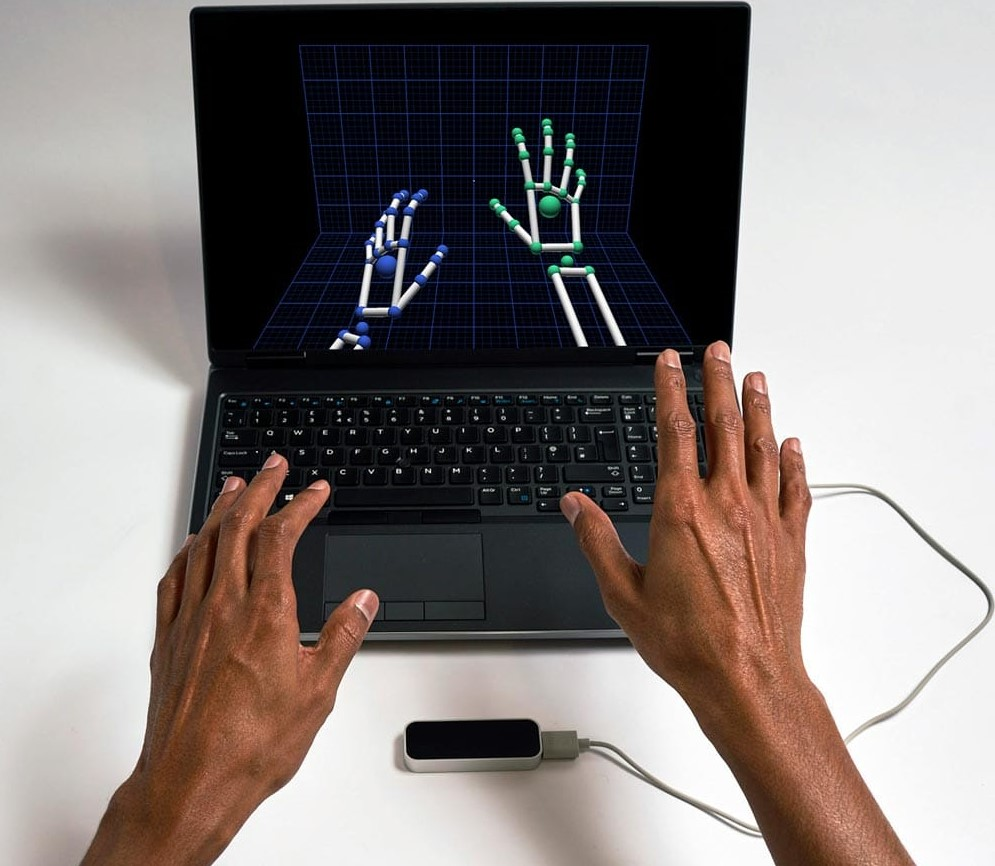
\includegraphics[width=0.6\textwidth]{figures/leapMotion.jpg}
\centering
\caption{Example of the Leap Motion tracking}
\label{fig:exampleLeap}
\end{figure}

In order to connect the existing Anonymous Panda prototype with the hand tracking part, it was necessary to use the official UE4 plugin, the Ultraleap Hand Tracking Plugin \cite{ULT}. This plugin allows Unreal developers to make use of the data obtained by incorporating Ultraleap's hand tracking data into their projects. It was designed with the intention of developing and implementing hand tracking in Extended Reality (XR) projects \cite{XR}, but with the right adjustments, it was possible to adapt its use to other types of projects \cite{ULTG}.

As mentioned, the Leap Motion Controller tracks hands and fingers with low latency and high precision, reporting position, velocity, and orientation. This controller may be placed on a VR headset or used on a tabletop. To incorporate Ultraleap's hand tracking data into a project, the Leap motion Controller system, which runs as a service or daemon, analyzes the images produced by its hardware and sends the analyzed data to the project. Then, the unreal plugin connected to the mentioned service converts the received data to the Unreal coordinate system. Furthermore, the plugin automatically transforms the tracking data to use a left-handed coordinate system and scales distance values to centimeters because the UE uses a left-handed convention for its coordinate system and centimeters as the default unit, whereas the Leap Motion uses a right-handed convention and millimeters as the default unit \cite{ULTP}. Figure \ref{fig:unrealAxes} shows the Unreal coordinate system in relationship to the Leap Motion device in Head Mounted Display (HMD) mode.

\begin{figure}[!htb]
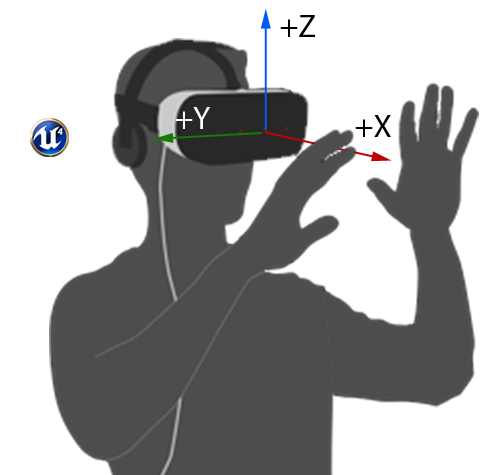
\includegraphics[width=0.3\textwidth]{figures/unrealAxes.png}
\centering
\caption{The Unreal coordinate system in relationship to the Leap Motion device in HMD mode}
\label{fig:unrealAxes}
\end{figure}

When the Leap Motion Controller has a good, high-contrast view of an object's silhouette, it uses infrared light and optical sensors to perform the detection and tracking work. These sensors have a $150^\circ$ field of view and their effective range extends from approximately 3 to 60 centimetres (Figure \ref{fig:HMDistance}). Last but not least, the Leap Motion software combines sensor data with an internal model of the human hand to handle complex tracking conditions \cite{ULTP}.

\begin{figure}[!htb]
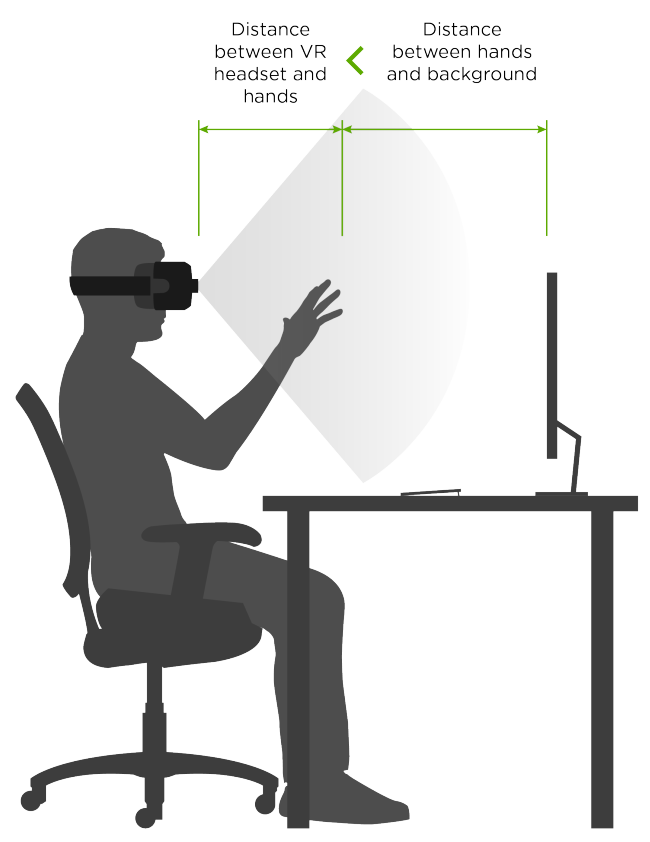
\includegraphics[width=0.4\textwidth]{figures/HMDistance.png}
\centering
\caption{In HMD mode, there should be less distance between the sensor and the hands than between the hands and any background objects or walls}
\label{fig:HMDistance}
\end{figure}

\subsubsection{The Hand Tracking Panda}
Because it is a useful, compact device that does not obstruct the face tracking component, we think the Leap Motion Controller is the ideal choice for this work. Therefore, in order to have the best performance in hand tracking, we chose to use the Leap Motion Controller in HMD mode because the Ultraleap Hand Tracking Plugin rotates the 3D hands to keep the correct orientation to the Unreal world when this mode is active \cite{ULTP}. In contrast with the Desktop Mounted Display (DMD) mode (Figure \ref{fig:DMD}), we can see that hand orientation in DMD mode is not ideal for our work since we want to track gestures, which are primarily vertical and happen while individuals are communicating with one another. This concern could be resolved by rotating the data gathered by the Leap Motion Controller before it is applied in the hands of the metahuman, however doing so would cause the prototype to perform slightly slower. We also decided to position the Leap Motion on the chest using a shirt clip made by a 3D printer, as shown in Figure \ref{fig:CMDvsHMD} (b) because using it on a VR support would obstruct the face tracking functionality (imagine having a VR headset as Figure \ref{fig:CMDvsHMD} (a) and wanting the metahuman to blink its right eye).

\begin{figure}[!htb]
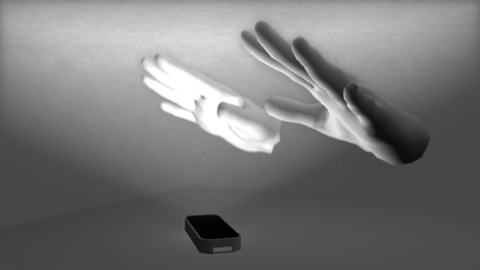
\includegraphics[width=0.6\textwidth]{figures/LeapView.jpg}
\centering
\caption{View of hands in DMD mode}
\label{fig:DMD}
\end{figure}

\begin{table}[!htb]
    \begin{minipage}{\linewidth}
        \centering
        \begin{subfigure}{0.49\textwidth}
            \centering
            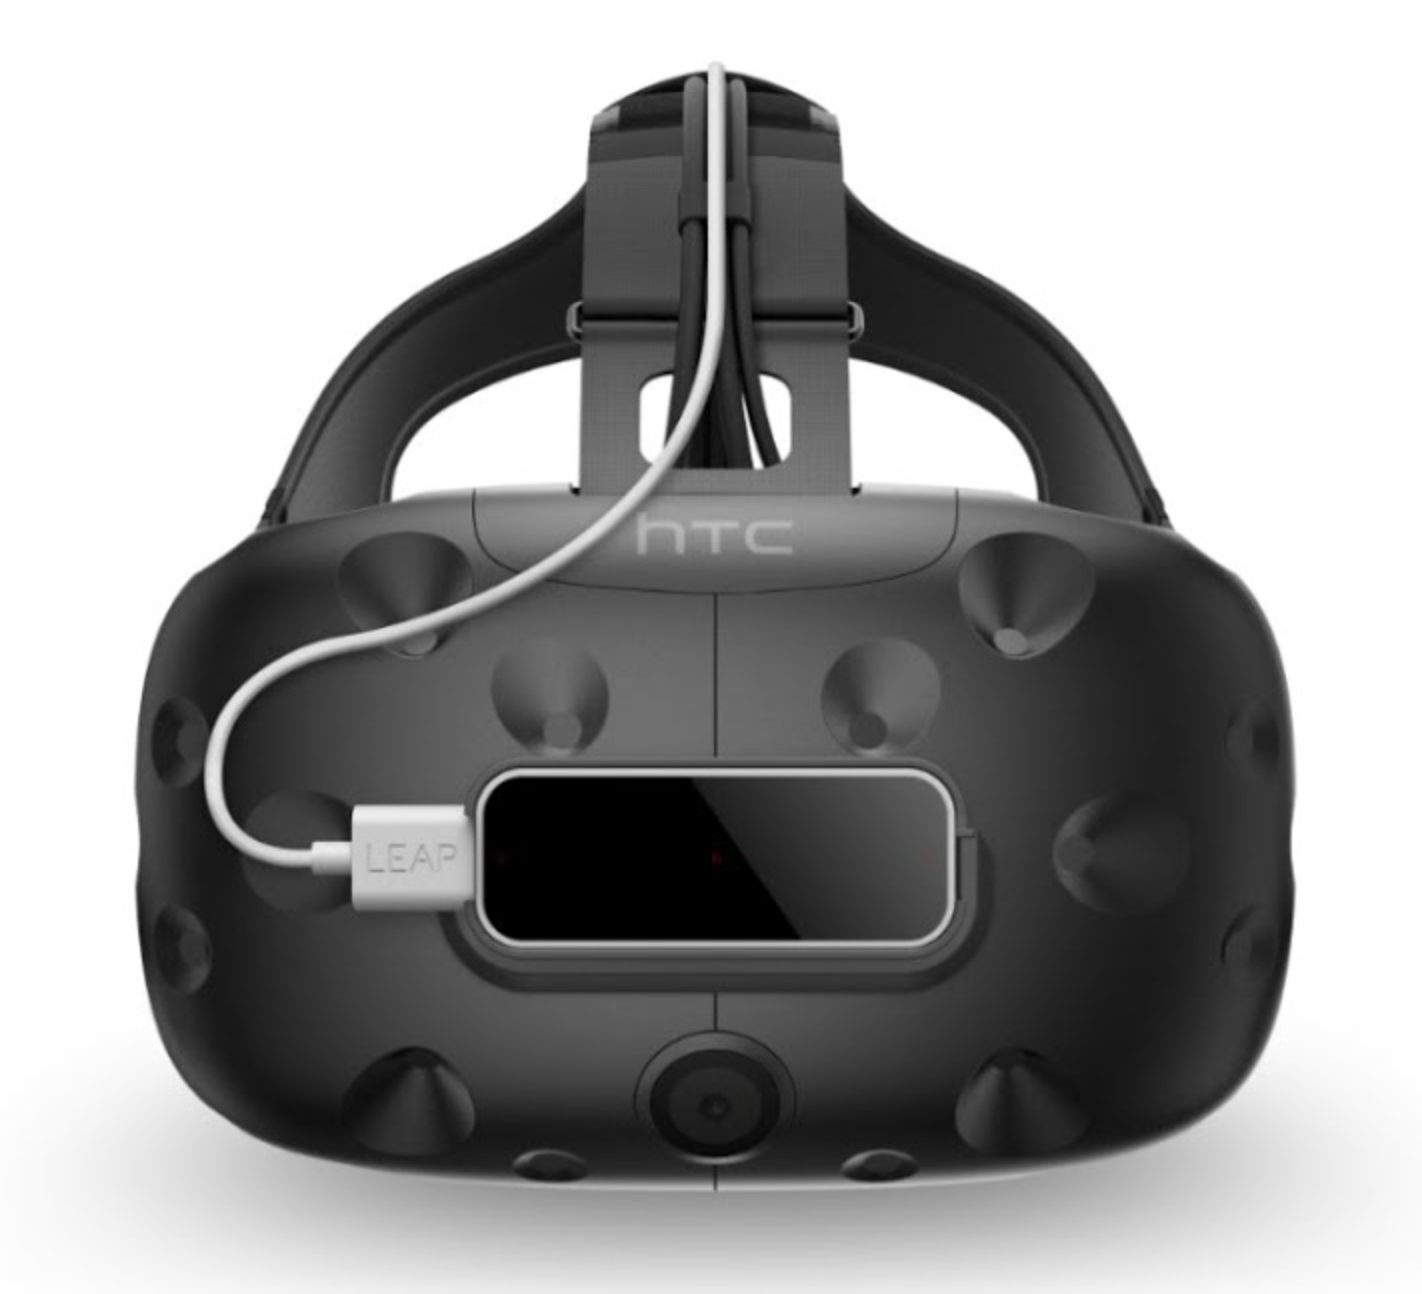
\includegraphics[width=\linewidth]{figures/VRsupport.png}
            \caption{Head (VR support)}
        \end{subfigure}
        \begin{subfigure}{0.49\textwidth}
            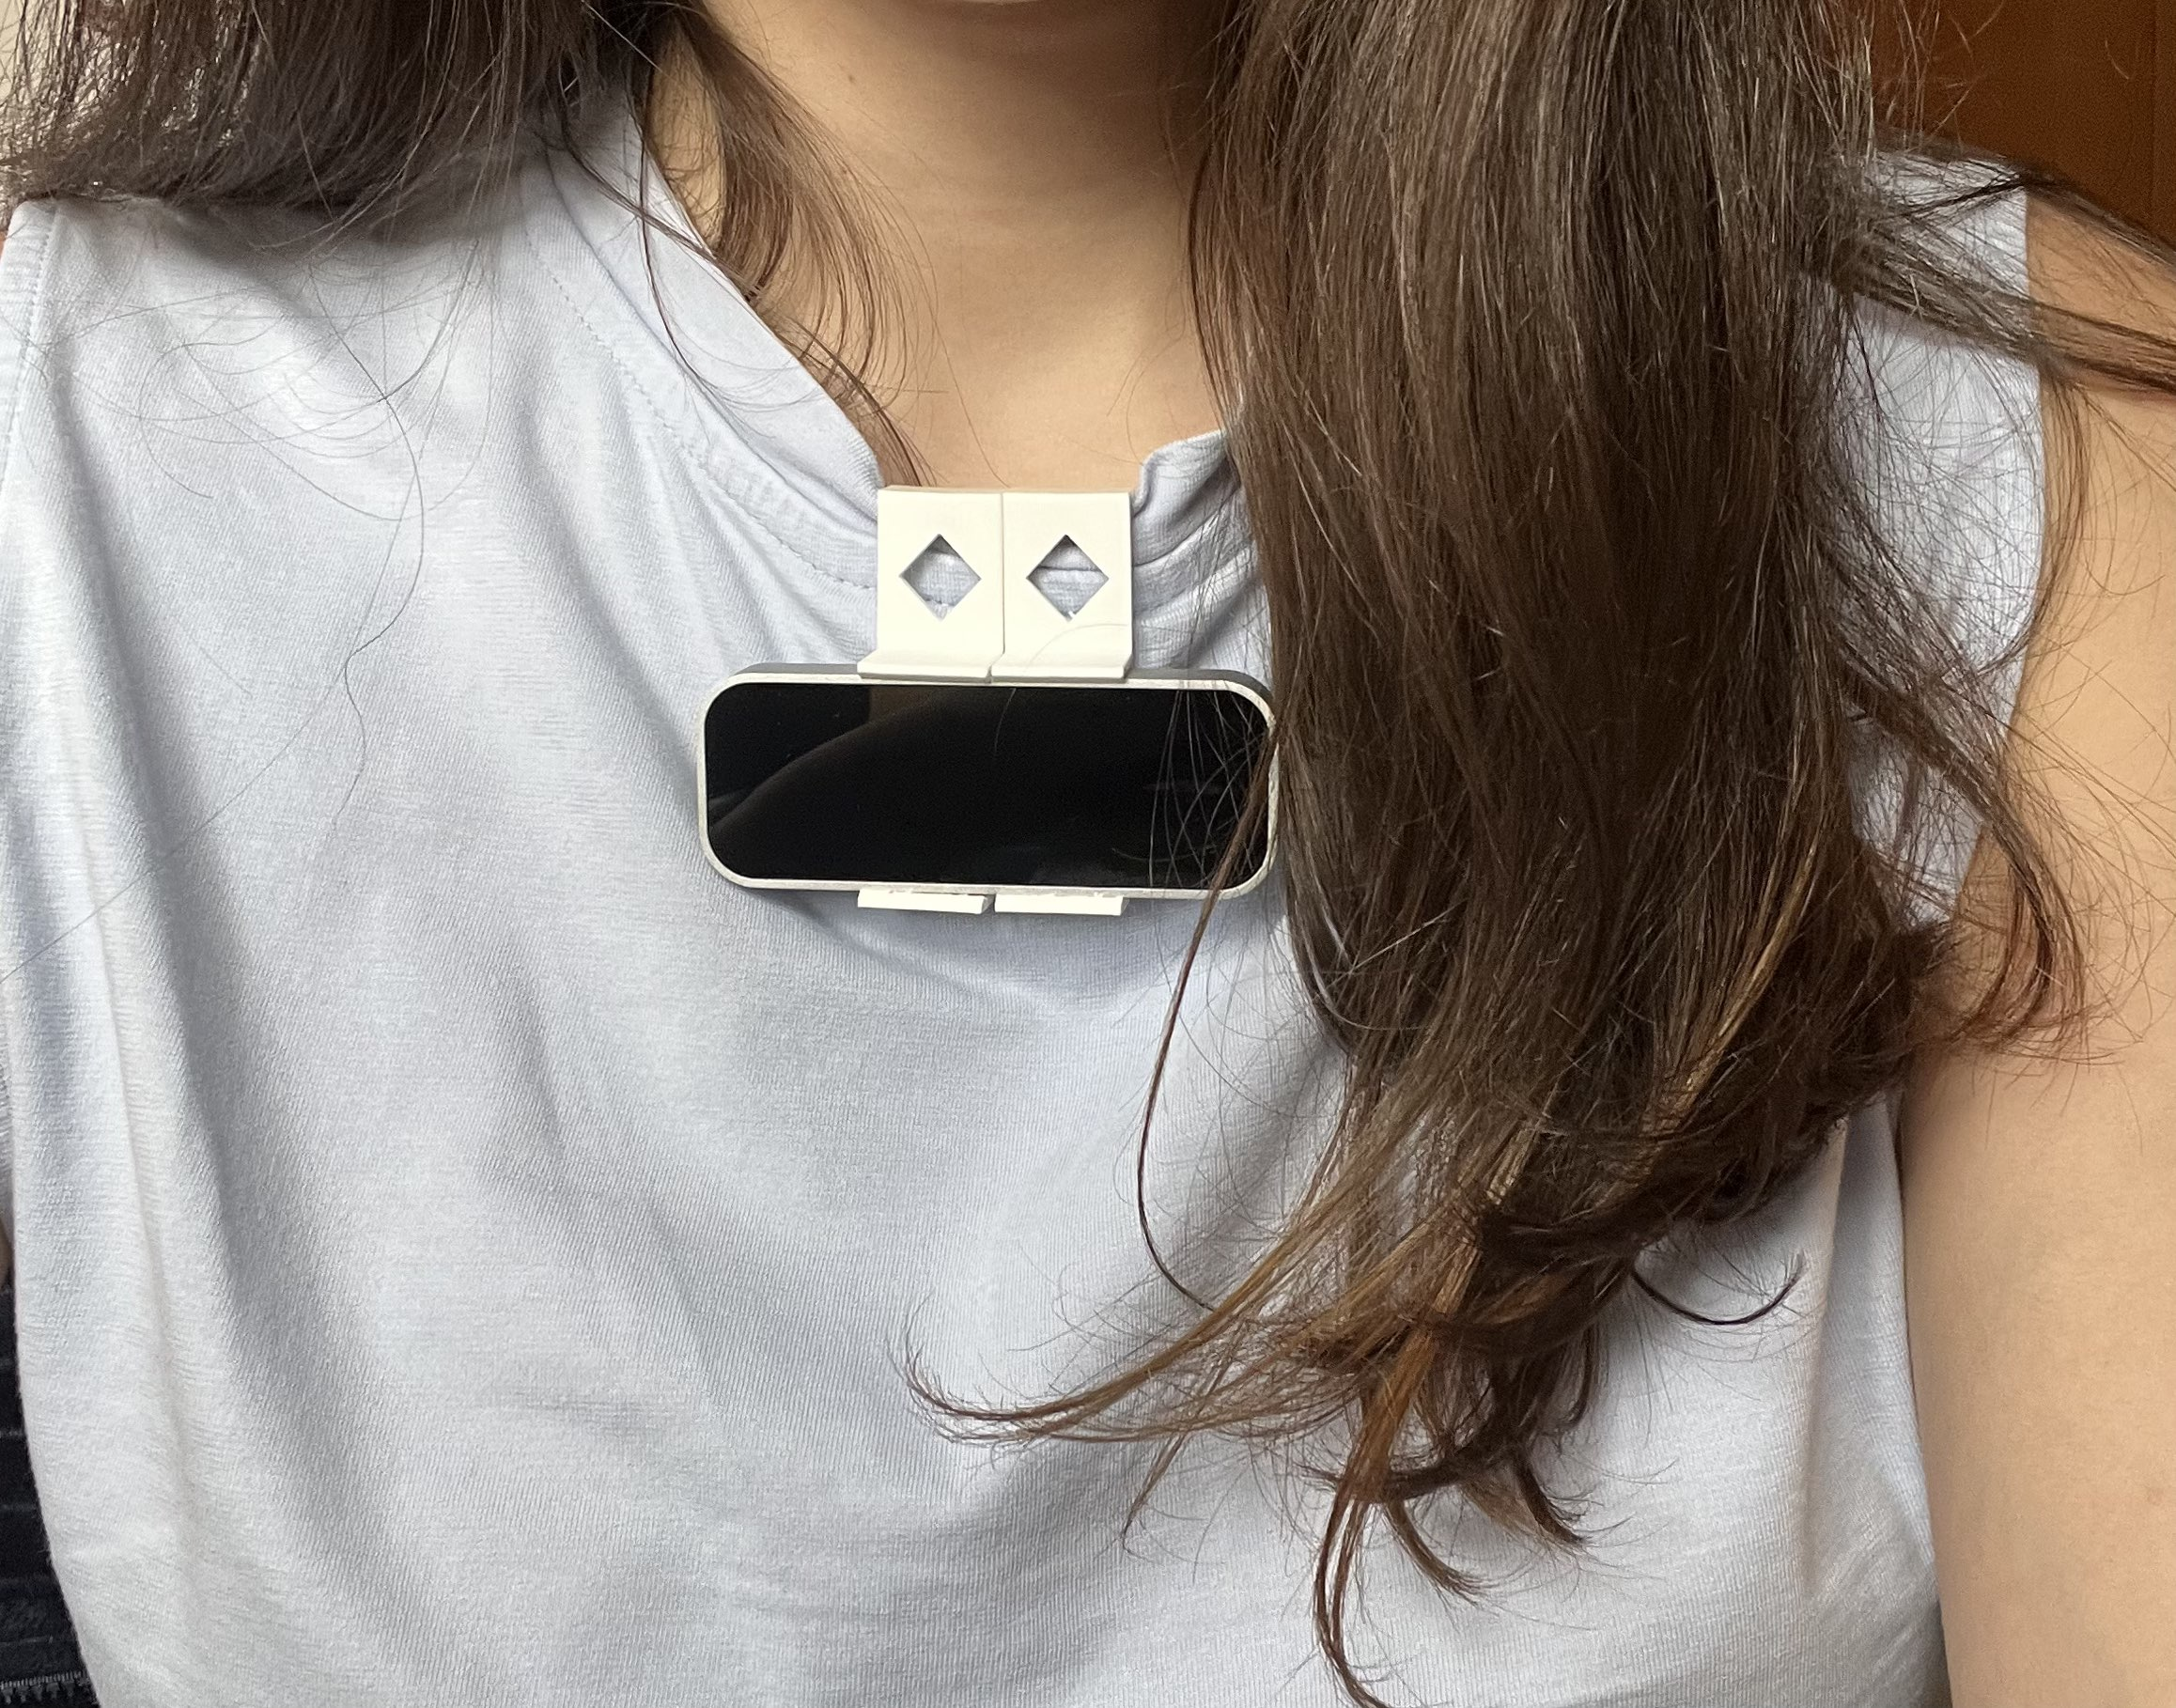
\includegraphics[width=\linewidth]{figures/CMD.jpg}
            \centering
            \caption{Chest}
        \end{subfigure}
        \captionof{figure}{Head vs. Chest Mounted Mode}
        \label{fig:CMDvsHMD}
	\end{minipage}
\end{table}

The official Ultraleap Tracking Plugin for Unreal Engine 4 utilizes pre-made blueprints to add hand tracking to a scene and play it in the editor. However, depending on the project, it may take a more customized approach using C\texttt{+}\texttt{+} or blueprints \cite{ULTGIT}. For our project, we attempted to adapt a custom rigging example map from the Ultraleap Plugin, which contained several animation blueprints \cite{LEAPMOD}, to create the new version of the Anonymous Panda prototype, beginning by seeing how each rigging was done and how we could adapt it to our metahumans' bones.

To use the rigging on our metahumans effectively, we had to re-parent the metahuman animation blueprint to "BodyStateAnimInstance". By utilizing the Body State system, we were able to map the tracked data collected by the Leap Motion Controller to the metahumans' skeletal mesh bones (Figure \ref{fig:mappedBones}).

\begin{table}[!htb]
    \begin{minipage}{\linewidth}
        \centering
        \begin{subfigure}{0.49\textwidth}
            \centering
            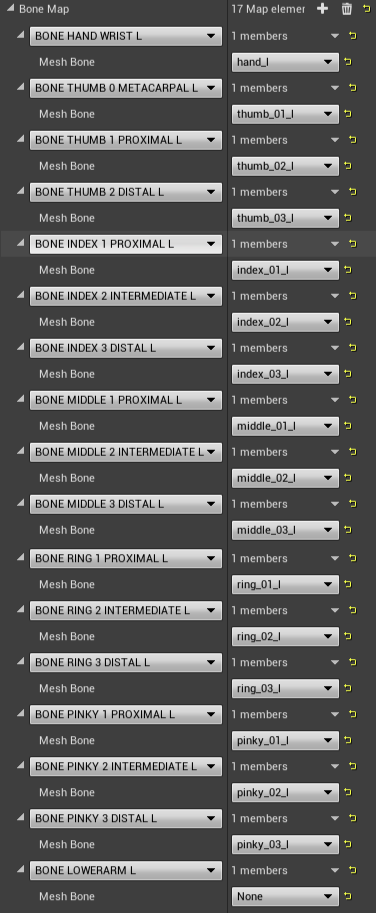
\includegraphics[width=\textwidth]{figures/mappedBones.png}
            \caption{Left Side}
        \end{subfigure}
        \begin{subfigure}{0.49\textwidth}
            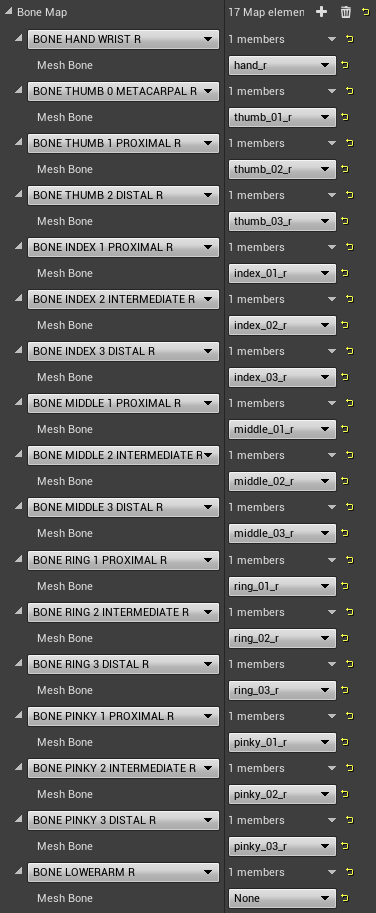
\includegraphics[width=\textwidth]{figures/mappedBonesR.png}
            \centering
            \caption{Right Side}
        \end{subfigure}
        \captionof{figure}{Tracked data mapped to the metahumans' skeletal hands mesh bones}
        \label{fig:mappedBones}
	\end{minipage}
\end{table}

We used the two Mapped Bone Anim Data arrays that were previously seen (Figure \ref{fig:mappedBones}), much like the two-handed example from the custom rigging map, and chose to disable the deformation mesh because the metahuman model does not yet allow deformation (Figure \ref{fig:mappedBoneList}).

\begin{figure}[!htb]
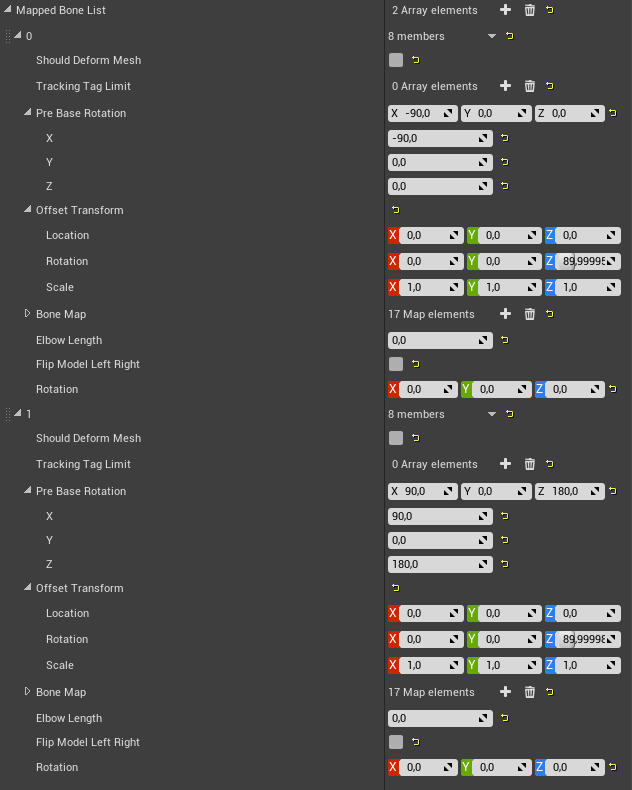
\includegraphics[width=0.8\textwidth]{figures/mappedBoneList.png}
\centering
\caption{Mapped Bone List}
\label{fig:mappedBoneList}
\end{figure}

Since we disabled the deformation mesh, only the rotations were tracked. To move the elbows to their proper positions, we apply an animation node called Forward And Backward Reaching Inverse Kinematics (FABRIK) to each elbow. The FABRIK animation node is an Inverse Kinematics (IK) solver that handles joint rotation from the location of an end-effector rather than directly from the joint rotation. In practice, we identify an effector location, and the IK solution solves the rotation so that the final joint is as close to that location as possible \cite{IK}.

Most animated skeletons in UE are powered by direct rotational data provided directly into the character's bones or the Skeletal Mesh. This is called Forward Kinematics (FK), or the direct application of rotation to joints or bones. Figure \ref{fig:diagramFK} illustrates a diagram of the concept.

\begin{figure}[!htb]
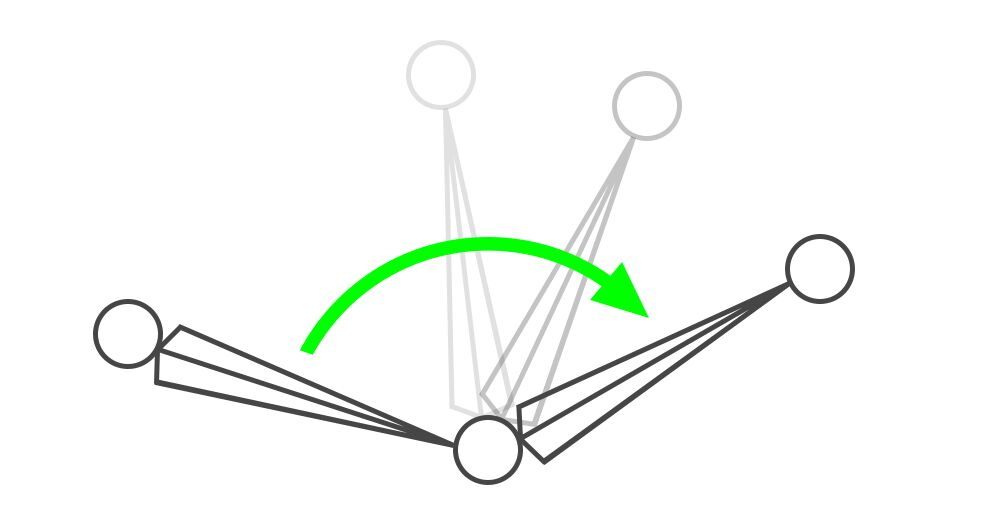
\includegraphics[width=0.8\textwidth]{figures/diagram_FK.png}
\centering
\caption{Forward Kinematics}
\label{fig:diagramFK}
\end{figure}

Meanwhile, Inverse Kinematics operates in the opposite direction. Instead of rotating bones, we provide the bone chain a target (also known as an end effector), specifying a position that the chain's end should aim for. The effector is moved by the user, and the IK solver (the algorithm that drives rotation in an IK system) rotates the bones so that the final bone in the chain ends at the target location \cite{IK}. The red cross in Figure \ref{fig:diagramIK} represents the end effector.

\begin{figure}[!htb]
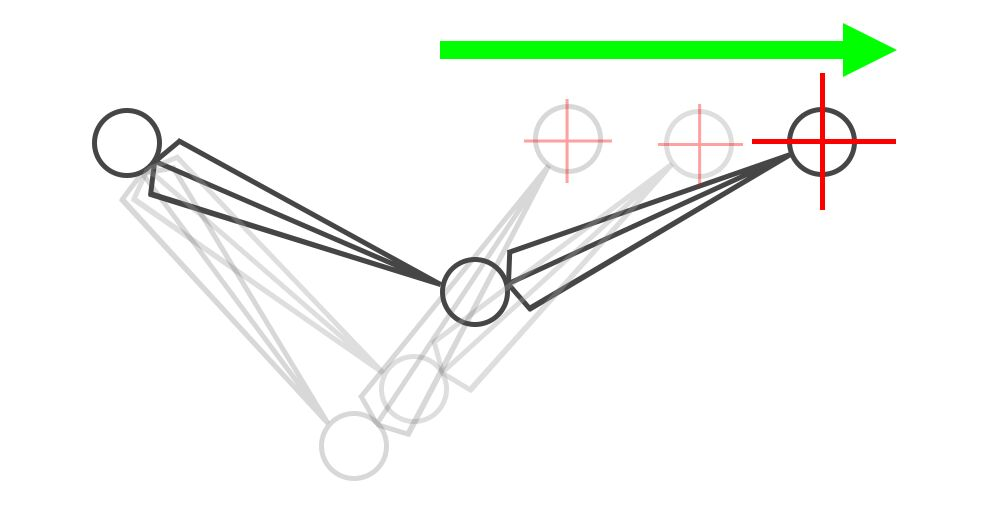
\includegraphics[width=0.8\textwidth]{figures/diagramIK.png}
\centering
\caption{Inverse Kinematics}
\label{fig:diagramIK}
\end{figure}

Once again, in order to position the shoulders correctly, we had to rotate all of our mapped data by 90 degrees in the "Offset Transform" for Y, as is typical for skeletal meshes and as shown in Figure \ref{fig:mappedBoneList}.

Concerning the prototype's outcome, Figure \ref{fig:BPHandsAndIK} depicts the steps taken from providing the IK with all of the data required for its operation to the metahuman's animation in the blueprint, after gathering data for the hands animation. Finally, Figure \ref{fig:handTrack} and videos \cite{APT1,APT2} illustrate the outcome applied to one of the metahumans used in this study.

\begin{figure}[!htb]
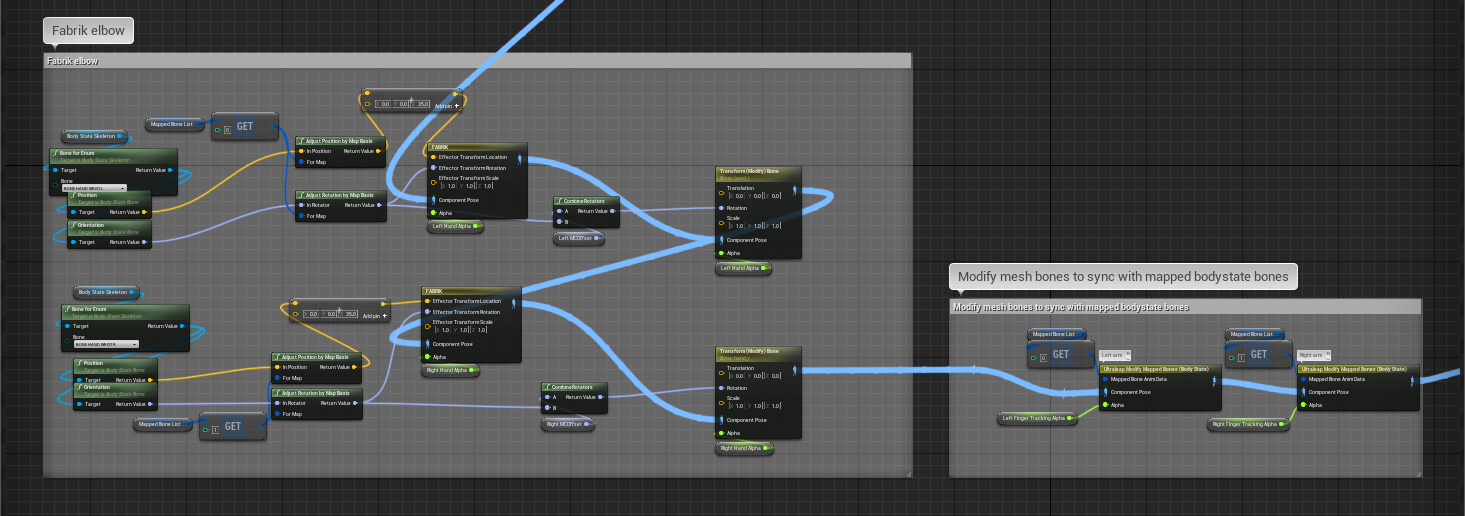
\includegraphics[width=\textwidth]{figures/BPHandsAndIK.png}
\centering
\caption{Blueprint in control of animating metahuman hands using data collected by leap motion}
\label{fig:BPHandsAndIK}
\end{figure}

\begin{figure}[!htb]
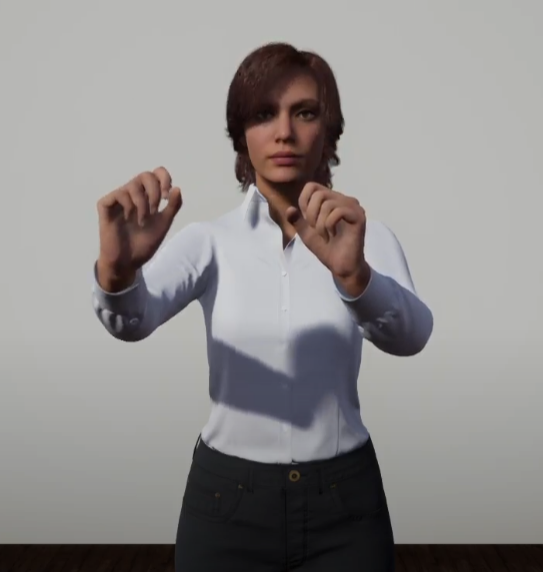
\includegraphics[width=0.5\textwidth]{figures/final.png}
\centering
\caption{The hand tracking's final outcome}
\label{fig:handTrack}
\end{figure}

\paragraph{Challenges}


\paragraph{Limitations}


% \subsection{Methodology}


% \subsubsection{Participants}


% \subsubsection{Procedure}


% \subsubsection{Hypotheses and Statistical Analyses}


% \subsubsection{Results}


% \subsubsection{Discussion}

